%%%%%%%%%%%%%%%%%%%%%%% file template.tex %%%%%%%%%%%%%%%%%%%%%%%%%
%
% This is a general template file for the LaTeX package SVJour3
% for Springer journals.          Springer Heidelberg 2010/09/16
%
% Copy it to a new file with a new name and use it as the basis
% for your article. Delete % signs as needed.
%
% This template includes a few options for different layouts and
% content for various journals. Please consult a previous issue of
% your journal as needed.
%
%%%%%%%%%%%%%%%%%%%%%%%%%%%%%%%%%%%%%%%%%%%%%%%%%%%%%%%%%%%%%%%%%%%
%
% First comes an example EPS file -- just ignore it and
% proceed on the \documentclass line
% your LaTeX will extract the file if required
\begin{filecontents*}{example.eps}
%!PS-Adobe-3.0 EPSF-3.0
%%BoundingBox: 19 19 221 221
%%CreationDate: Mon Sep 29 1997
%%Creator: programmed by hand (JK)
%%EndComments
gsave
newpath
  20 20 moveto
  20 220 lineto
  220 220 lineto
  220 20 lineto
closepath
2 setlinewidth
gsave
  .4 setgray fill
grestore
stroke
grestore
\end{filecontents*}
%
\RequirePackage{fix-cm}
%
%\documentclass{svjour3}                     % onecolumn (standard format)
%\documentclass[smallcondensed]{svjour3}     % onecolumn (ditto)
\documentclass[smallextended]{svjour3}       % onecolumn (second format)
%\documentclass[twocolumn]{svjour3}          % twocolumn
%
\smartqed  % flush right qed marks, e.g. at end of proof
%
\usepackage{graphicx}
%
% \usepackage{mathptmx}      % use Times fonts if available on your TeX system
%
% insert here the call for the packages your document requires
%\usepackage{latexsym}
% etc.
%
% please place your own definitions here and don't use \def but
% \newcommand{}{}
%
% Insert the name of "your journal" with
% \journalname{myjournal}
%
\begin{document}

\title{Breast milk on the go:%\thanks{Grants or other notes
%about the article that should go on the front page should be
%placed here. General acknowledgments should be placed at the end of the article.}
}
\subtitle{Postpartum mobility of Twe women}

%\titlerunning{Short form of title}        % if too long for running head

\author{Layne Vashro
}

%\authorrunning{Short form of author list} % if too long for running head

\institute{L. Vashro \at
              270 South 1400 East, Salt Lake City, UT 84112 \\
              Tel.: +001 (801) 581 6251\\
              \email{layne.vashro@anthro.utah.edu}           %  \\
}

\date{Received: date / Accepted: date}
% The correct dates will be entered by the editor


\maketitle

\begin{abstract}
Insert your abstract here. Include keywords, PACS and mathematical
subject classification numbers as needed.
\keywords{First keyword \and Second keyword \and More}
% \PACS{PACS code1 \and PACS code2 \and more}
% \subclass{MSC code1 \and MSC code2 \and more}
\end{abstract}

\section{Introduction}
\label{sec:1}
<<<<<<< HEAD
<<<<<<< HEAD
Your text comes here. Separate text sections with

Researchers consistently find sex-differences in spatial-cognitive and navigational tasks, as well as measures of geographical range of movement.  These differences are well-documented in Western industrialized societies and have increasingly been replicated cross-culturally.  Psychologists have proposed several different theories linking these sex differences into a cohesive evolutionary story.  Ancestral males who traveled more safely and effectively long-distance and into unfamiliar terrain in search of mates, game, or batter (cite, cite, cite) were paid in fitness.  This selected for superior navigation ability and the underlying spatial-cognitive traits that facilitate navigational performance.  However, not all evolutionary explanations for this cluster of sex differences focuses on adaptive advantages in men.  Sherry and Hampson (cite) are consistent with the other theories, but rather than focus on men looks at the fitness ramifications of women's long-distance mobility.  This ``fertility and parental care hypothesis'' explains the observed sex differences in terms of the potential costs to women traveling, particularly during key period of reproduction.
=======
Researchers consistently find sex-differences in spatial-cognitive and navigational tasks, as well as measures of geographical range of movement.  These differences are well-documented in Western industrialized societies and have increasingly been replicated cross-culturally, including among uneducated populations.  Evolutionary psychologists have put forward a number of different theories that link the sex differences in these traits into a single cohesive story.  In most of these theories, past selection favored males who were better are traveling long distances and into unknown environments (with the payoff of that travel, mates/hunting/warfare being the key point of discrimination) and this required superior navigation ability and the spatial-cognitive traits that facilitate it.  However, one explanation for these differences ignores the payoffs to males and instead turns the focus on the fitness ramifications of women's long-distance mobility.  This ``fertility and parental care hypothesis'' put forward by ... argues that the observed sex differences can be explained in terms of the potential costs to women traveling, particularly during key period of reproduction.
>>>>>>> parent of 97f05c4... anth chnages this morning

=======
Your text comes here. Separate text sections with
>>>>>>> parent of 02eeed8... plane work
	\subsection{Fertility and parental care}
	\label{sec:1.1}
Simple description of the fertility and parental care hypothesis.

Particular issues.  Cambell and ``staying alive''... segue into issues of infanticide and rape...  Caloric expenditure

Mechanism: i.e. mediated by estrogen and probably other stuff.

	\subsection{Post-partum hormones and spatial ability}
	\label{sec:1.2}
Awkwardly, the post-partum period, when women are dealing with very young and dependent offspring is actually a period of decreased estrogen.  Mice stuff...

\section{Methods}
\label{sec:2}
Text with citations \cite{RefB} and \cite{RefJ}.
	\subsection{Mobility interviews}
	\label{sec:2.1}
Your text comes here. Separate text sections with	
	\subsection{Spatial cognition}
	\label{sec:2.2}
Your text comes here. Separate text sections with

\section{Results}
\label{sec:3}
Text with citations \cite{RefB} and \cite{RefJ}.
	\subsection{Mobility interviews}
	\label{sec:3.1}
Your text comes here. Separate text sections with	

% For one-column wide figures use
\begin{figure}
  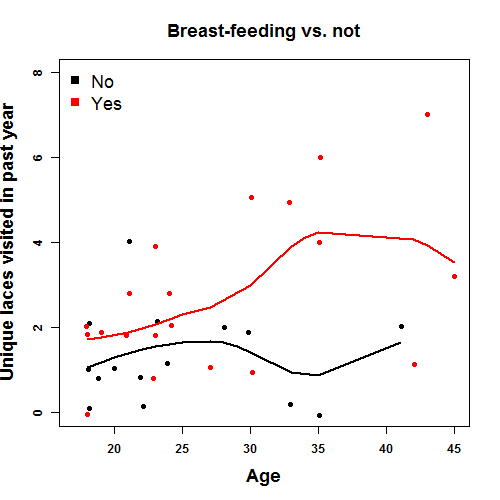
\includegraphics[width=0.75\textwidth]{bfeed_mob}
\caption{Please write your figure caption here}
\label{fig:1}       % Give a unique label
\end{figure}

	\subsection{Spatial cognition}
	\label{sec:3.2}
Your text comes here. Separate text sections with

\section{Discussion}
\label{sec:4}
Text with citations \cite{RefB} and \cite{RefJ}.

%
% For two-column wide figures use
\begin{figure*}
  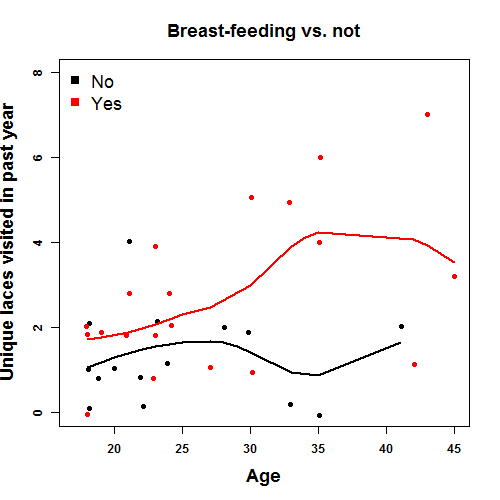
\includegraphics[width=0.75\textwidth]{bfeed_mob}
\caption{Please write your figure caption here}
\label{fig:2}       % Give a unique label
\end{figure*}
%
% For tables use
\begin{table}
% table caption is above the table
\caption{Please write your table caption here}
\label{tab:1}       % Give a unique label
% For LaTeX tables use
\begin{tabular}{lll}
\hline\noalign{\smallskip}
first & second & third  \\
\noalign{\smallskip}\hline\noalign{\smallskip}
number & number & number \\
number & number & number \\
\noalign{\smallskip}\hline
\end{tabular}
\end{table}


%\begin{acknowledgements}
%If you'd like to thank anyone, place your comments here
%and remove the percent signs.
%\end{acknowledgements}

% BibTeX users please use one of
%\bibliographystyle{spbasic}      % basic style, author-year citations
%\bibliographystyle{spmpsci}      % mathematics and physical sciences
%\bibliographystyle{spphys}       % APS-like style for physics
%\bibliography{}   % name your BibTeX data base

% Non-BibTeX users please use
\begin{thebibliography}{}
%
% and use \bibitem to create references. Consult the Instructions
% for authors for reference list style.
%
\bibitem{RefJ}
% Format for Journal Reference
Author, Article title, Journal, Volume, page numbers (year)
% Format for books
\bibitem{RefB}
Author, Book title, page numbers. Publisher, place (year)
% etc
\end{thebibliography}

\end{document}
% end of file template.tex

